\documentclass[11pt]{article}
%Homework 01 |065|=)

\usepackage{amsmath,amssymb}
\usepackage{graphicx}
\usepackage[colorlinks=true,citecolor=black,linkcolor=black,urlcolor=blue]{hyperref}
\usepackage{tikz,graphics,color,fullpage,float,epsf,caption,subcaption}
\usepackage[utf8]{inputenc}

\title{\textbf{Plynomial Systems Solving}}
\author{Burak ŞENER\\
        Mehmet PEKMEZCİ\\
		Mustafa Mert ERGİN
		}
\date{}
\begin{document}
\maketitle
\begin{abstract}
\emph{This work is a survey on the subject Polynomial Systems Solving. First , Polynomial Systems definition is studied , then their solution techniques are studied, finally application areas are discussed. }
\end{abstract}

\section{Introduction}

\subsection{Polynomial}
 A polynomial is a mathematical expression involving a sum of powers in one or more variables (indeterminates) multiplied by coefficients. A polynomial of order/degree $\mathbf{d}$  in one variable (x)  (i.e., a univariate polynomial) with constant coefficients ($\mathbf{a_i}$) is given by \cite{wolframPolynomial}
\begin{equation}
    a_{0}+a_{1}x+a_{2}{x}^2+\cdots+a_{d}{x}^d 
\end{equation}

A polynomial may not have a term with negative and fractional exponent ($\mathrm{x^{-n}}$ and $\mathrm{x^{1/n}}$ ). Every term ( $\mathbf{a_ix^i}$ ) may be called as monomial (in some books only $\mathbf{x^i}$ is called as monomial). Also in abstract algebra books,  a \textbf{Polynomial} is called as \textbf{Polynomial Ring}. Abstract algebraic notions are explained in the next section.

\subsection{Polynomial System}

A system of (multivariate) polynomial equations is a set of simultaneous equations $\mathrm{f_{1}}$  = 0, ..., $\mathrm{f_{m}}$ = 0 where the $\mathrm{f_{i}}$ are polynomials in several variables, say $\mathrm{x_{1}}$, ..., $\mathrm{x_{n}}$, over some field k (usually $\mathbb{C}$ or $\mathbb{R}$ ). \cite{wikipediaSystemofPolynomialEquations}. 

A \textbf{Univariate Polynomial System}  (coefficients  $\mathrm{a_{ij} \in R}$  and i,j,n $\mathrm{\in N}$) may be given as : 

\begin{equation}  
   \begin{cases}
    a_{10}+a_{11}x+a_{12}x^2+a_{13}x^3+a_{14}x^4+\ldots+a_{1d}x^d=0 \\
    a_{20}+a_{21}x+a_{22}x^2+a_{13}x^3+a_{14}x^4+\ldots+a_{2d}x^d=0 \\
    a_{30}+a_{31}x+a_{12}x^2+a_{13}x^3+a_{14}x^4+\ldots+a_{3d}x^d=0 \\
    \vdots \\
    a_{m0}+a_{m1}x+a_{m2}x^2+a_{m3}x^3+a_{m4}x^4+\ldots+a_{md}x^d=0 \\
  \end{cases}
\end{equation}

A \textbf{Bivariate Polynomial System}  (variables  $\mathrm{x,y \in R}$ ,  coefficients  $\mathrm{a_{ij} \in R}$  and i,j,n $\mathrm{\in N}$) may be given as : 

\begin{equation}  
   \begin{cases}
    a_{10}+a_{11} {x_1}^{k_{11}} {x_2}^{k_{12}}\ldots+a_{12}{x_1}^{k_{11}} {x_2}^{k_{12}}\ldots+a_{13}x^3+a_{14}x^4+\ldots+a_{1d}x^d=0 \\
    a_{20}+a_{21}x+a_{22}x^2+a_{13}x^3+a_{14}x^4+\ldots+a_{2d}x^d=0 \\
    a_{30}+a_{31}x+a_{12}x^2+a_{13}x^3+a_{14}x^4+\ldots+a_{3d}x^d=0 \\
    \vdots \\
    a_{m0}+a_{m1}x+a_{m2}x^2+a_{m3}x^3+a_{m4}x^4+\ldots+a_{md}x^d=0 \\
  \end{cases}
\end{equation}



\begin{figure}[h!]
  \centering
  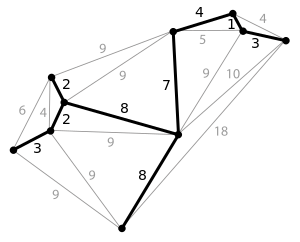
\includegraphics[width=0.4\linewidth]{spanning.png}
  \caption[Spanning Tree of a graph G ]{Spanning Tree of a graph G \footnotemark}
  \label{fig:spanningTree}
\end{figure}
\footnotetext{\url{https://en.wikipedia.org/wiki/Minimum_spanning_tree}}

\section{Previous Work}
Minimum Spanning Tree of an undirected and weighted graph G , is the spanning tree of G with the minimum  total edge weights. \footnote{http://www.scielo.br/scielo.php?script=sci\_arttext\&pid=S0101-74382005000200004} There are a lot of algorithms finding M.S.T. of a graph, including Kruskal ve Prim algorithms. 
 
\section{Conclusion}
Kruskal and Prim algorithms finds the minimum spanning tree, but if we want to find all spanning trees , several algorithms exist (e.g. Gabow \& Myers, 1978; Kapoor \& Ramesh, 1995; Matsui, 1993; Minty, 1965; Shioura \& Tamura, 1995; Read \& Tarjan, 1975; Kapoor \& Ramesh, 2000; Matsui, 1997). Good space and time complexities are the most important concerns of these algorithms. Most algorithms generate spanning trees using some fundamental cut or circuit, but none of them takes the cost of the tree into account while generating spanning trees, except Kenneth SORENSEN  and  Gerrit K. JANSSENS,  with the article "An algorithm to generate all spanning trees of a graph in order of increasing cost. Pesqui. Oper. [online]. 2005, vol.25, n.2" . In this article they generate all spanning trees in order of increasing cost.

There is a recent paper that uses divide and conquer algorithm to find all spanning trees of a graph which is called DCC\_Trees. (Chakraborty, Maumita \& Hazra, Goutam \& Pal, Rajat. (2018). Divide-and-Conquer: An Approach to Generate All Spanning Trees of a Connected and Undirected Simple Graph)\footnote{http://www.springer.com/cda/content/document/cda\_downloaddocument/9789811034084\-c2.pdf}

\begin{figure}[h!]
  \centering
  \begin{subfigure}[b]{0.4\linewidth}
    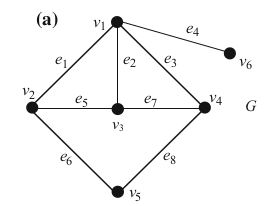
\includegraphics[width=\linewidth]{graph0.png}
    \caption{Graph G.}
  \end{subfigure} 
  \begin{subfigure}[b]{0.4\linewidth}
    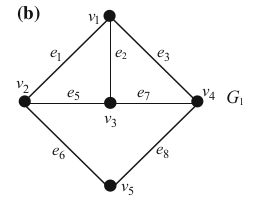
\includegraphics[width=\linewidth]{graph1.png}
    \caption{$\mathrm{G_{1}}$ = G - \{$\mathrm{e_{4}}$\}.}
  \end{subfigure}
  \caption[Partitions]{Partitions of a graph G \footnotemark}
  \label{fig:coffee1}
\end{figure}\footnote{http://www.springer.com/cda/content/document/cd\_downloaddocument/9789811034084\-c2.pdf}

DCC\_Trees algorithm is as follows : 

\begin{enumerate}
\item Divide : Divide the graph into primary and secondary partitions
	\begin{enumerate}
		\item Primary Partition : All possible combinations of the edges coming out from the reference vertex, $\mathrm{v_{ref}}$ , taken one to all at a time, form the primary partitions in this algorithm.
		\item Secondary Partition  : Once a primary partition is selected, one or more vertices, other than the $\mathrm{v_{ref}}$ , also get included or visited.
	\end{enumerate}
\item Conquer : Searching for Connectors. 
\item Combine : Forming the Trees
\end{enumerate}


Finiteness of the algorithm can be proven by saying that we have limited number of edges/vertices's.

Correctness of the algorithm is proven by the two theorems within the paper. 

\cite[chapter 2, p.~215]{wolframPolynomial}


\section{Conlusion}
Total number of spanning trees are calculated using  Kirchhoff’s Theorem.\footnote{https://www.geeksforgeeks.org/total-number-spanning-trees-graph/}
\footnote{https://en.wikipedia.org/wiki/Kirchhoff\%27s\_theorem\#Proof\_outline}


\begin{thebibliography}{1}
\bibitem{berndStrumfelsBook}
  Strumfels Bernd,
  \textit{Solving Systems of Polynomial Equations},
   American Mathematical Society , Conference Board of Mathematical Sciences,
   Berkeley,CA,
   2002.
\bibitem{dineshManocaArticle}
  Manocha Dinesh,
  \textit{Solving Systems of Polynomial Equations},
   IEEE Computer Graphics and Applications
   University of North Carolina,
   1994.
\bibitem{hybridMethodArticle}
  L.H. Zhi and Y. Notake and H. Kai and M.-T. Noda and K.I. Shiraishi,
  \textit{Hybrid Method for Solving Polynomial Equations},
   Proceedings of the Asian Technology Conference in Mathematics, pp.492-501, Guangzhou, China, 1999. 
\bibitem{gregoryBardThesis}
  Bard Gregory,
  \textit{Algorithms for Solving Linear and Polynomial Systems of Equations Over Finite Fields With Applications to Cryptanalysis},
   University of Maryland PHD Thesis,
   2007.
\bibitem{dineshManocaArticle}
  Luk Bettale 1 , Jean-Charles Faugère, Ludovic Perret,
  \textit{Solving multivariate polynomial systems over finite fields : Hybrid approach},
   Journées Nationales du Calcul Formel,
   UPMC, CNRS, INRIA Paris-Rocquencourt,
   2002.
   
\bibitem{dineshManocaArticle}
  Manocha Dinesh,
  \textit{Solving Systems of Polynomial Equations},
   IEEE Computer Graphics and Applications
   University of North Carolina,
   1994.
\bibitem{dineshManocaArticle}
  Manocha Dinesh,
  \textit{Solving Systems of Polynomial Equations},
   IEEE Computer Graphics and Applications
   University of North Carolina,
   1994.
\bibitem{dineshManocaArticle}
  Manocha Dinesh,
  \textit{Solving Systems of Polynomial Equations},
   IEEE Computer Graphics and Applications
   University of North Carolina,
   1994.
\bibitem{dineshManocaArticle}
  Manocha Dinesh,
  \textit{Solving Systems of Polynomial Equations},
   IEEE Computer Graphics and Applications
   University of North Carolina,
   1994.
\bibitem{dineshManocaArticle}
  Manocha Dinesh,
  \textit{Solving Systems of Polynomial Equations},
   IEEE Computer Graphics and Applications
   University of North Carolina,
   1994.
\bibitem{dineshManocaArticle}
  Manocha Dinesh,
  \textit{Solving Systems of Polynomial Equations},
   IEEE Computer Graphics and Applications
   University of North Carolina,
   1994.
\bibitem{dineshManocaArticle}
  Manocha Dinesh,
  \textit{Solving Systems of Polynomial Equations},
   IEEE Computer Graphics and Applications
   University of North Carolina,
   1994.
\bibitem{dineshManocaArticle}
  Manocha Dinesh,
  \textit{Solving Systems of Polynomial Equations},
   IEEE Computer Graphics and Applications
   University of North Carolina,
   1994.
\bibitem{dineshManocaArticle}
  Manocha Dinesh,
  \textit{Solving Systems of Polynomial Equations},
   IEEE Computer Graphics and Applications
   University of North Carolina,
   1994.
\bibitem{dineshManocaArticle}
  Manocha Dinesh,
  \textit{Solving Systems of Polynomial Equations},
   IEEE Computer Graphics and Applications
   University of North Carolina,
   1994.
\bibitem{dineshManocaArticle}
  Manocha Dinesh,
  \textit{Solving Systems of Polynomial Equations},
   IEEE Computer Graphics and Applications
   University of North Carolina,
   1994.
\bibitem{dineshManocaArticle}
  Manocha Dinesh,
  \textit{Solving Systems of Polynomial Equations},
   IEEE Computer Graphics and Applications
   University of North Carolina,
   1994.
\bibitem{dineshManocaArticle}
  Manocha Dinesh,
  \textit{Solving Systems of Polynomial Equations},
   IEEE Computer Graphics and Applications
   University of North Carolina,
   1994.
\bibitem{dineshManocaArticle}
  Manocha Dinesh,
  \textit{Solving Systems of Polynomial Equations},
   IEEE Computer Graphics and Applications
   University of North Carolina,
   1994.
\bibitem{dineshManocaArticle}
  Manocha Dinesh,
  \textit{Solving Systems of Polynomial Equations},
   IEEE Computer Graphics and Applications
   University of North Carolina,
   1994.
\bibitem{wikipediaSystemofPolynomialEquations}
  \textit{ https://en.wikipedia.org/wiki/System\_of\_polynomial\_equations},
   Wikipedia,2018.
   
\bibitem{wolframPolynomial}
  \textit{ http://mathworld.wolfram.com/Polynomial.html},
   Wolfram,2018.

\end{thebibliography}

\end{document}



